\documentclass[12pt, titlepage]{article}

\usepackage{fullpage}
\usepackage[round]{natbib}
\usepackage{multirow}
\usepackage{booktabs}
\usepackage{tabularx}
\usepackage{graphicx}
\usepackage{float}
\usepackage{hyperref}
\usepackage{colortbl}
\usepackage[table]{xcolor} 
\hypersetup{
    colorlinks,
    citecolor=blue,
    filecolor=black,
    linkcolor=red,
    urlcolor=blue
}

%% Comments

\usepackage{color}

%\newif\ifcomments\commentstrue %displays comments
\newif\ifcomments\commentsfalse %so that comments do not display

\ifcomments
\newcommand{\authornote}[3]{\textcolor{#1}{[#3 ---#2]}}
\newcommand{\todo}[1]{\textcolor{red}{[TODO: #1]}}
\else
\newcommand{\authornote}[3]{}
\newcommand{\todo}[1]{}
\fi

\newcommand{\wss}[1]{\authornote{blue}{SS}{#1}} 
\newcommand{\plt}[1]{\authornote{magenta}{TPLT}{#1}} %For explanation of the template
\newcommand{\an}[1]{\authornote{cyan}{Author}{#1}}

%% Common Parts

\newcommand{\progname}{Mechatronics Engineering} % PUT YOUR PROGRAM NAME HERE
\newcommand{\authname}{Team 25, Preliminary
\\ Ahmed Nazir, nazira1
\\ Stephen Oh, ohs9
\\ Muhanad Sada, sadam
\\ Tioluwalayomi Babayeju, babayejt} % AUTHOR NAMES                  

\usepackage{hyperref}
    \hypersetup{colorlinks=true, linkcolor=blue, citecolor=blue, filecolor=blue,
                urlcolor=blue, unicode=false}
    \urlstyle{same}
                                


\newcounter{acnum}
\newcommand{\actheacnum}{AC\theacnum}
\newcommand{\acref}[1]{AC\ref{#1}}

\newcounter{ucnum}
\newcommand{\uctheucnum}{UC\theucnum}
\newcommand{\uref}[1]{UC\ref{#1}}

\newcounter{mnum}
\newcommand{\mthemnum}{M\themnum}
\newcommand{\mref}[1]{M\ref{#1}}

\begin{document}

\title{System Design for \progname{}} 
\author{\authname}
\date{\today}

\maketitle

\pagenumbering{roman}

\section{Revision History}

\begin{tabularx}{\textwidth}{p{3cm}p{2cm}X}
\toprule {\bf Date} & {\bf Version} & {\bf Notes}\\
\midrule
2023/01/14 & 1.0 & General Updates\\
2023/01/18 & 2.0 & Final Version\\
\bottomrule
\end{tabularx}

\newpage

\section{Reference Material}

This section records information for easy reference.

\subsection{Abbreviations and Acronyms}

\renewcommand{\arraystretch}{1.2}
\begin{tabular}{l l} 
  \toprule		
  \textbf{symbol} & \textbf{description}\\
  \midrule 
  \progname & Mechatronics Engineering Capstone Course\\
  UART & Universal Asynchronous Receiver-Transmitter\\
  SPI & Serial Peripheral Interface\\
  I2C & Inter-Integrated Circuit\\
  USB & Universal Serial Bus\\
  TCP & Transmission Control Protocol\\
  IP & Internet Protocol\\
  SPDT & Single pole, double throw \\
  TCP/IP & Transmission Control Protocol / Internet Protocol \\
  SOC & Software On Chip \\
  SPST & Single pole, single throw \\
  TX & Transmit \\
  RX & Recieve \\
  USB & Universal Serial Bus \\
  LED & Light-emitting diode \\
  GB & GigaByte \\
  SD & Secure Digital \\
  PCB & Printed Circuit Board \\
  \bottomrule
\end{tabular}\\

\newpage

\tableofcontents

\newpage

\listoftables

\listoffigures

\newpage

\pagenumbering{arabic}

\section{Introduction}

The system design document establishes the group's development considerations for the Formulate system. The motivations which drove each aspect of the design were referenced back to the System Requirements Specification, Hazard Analysis, and Development Plan documents. 

\wss{Include references to your other documentation}

\section{Purpose}

\wss{Purpose of your design documentation}

\wss{Point to your other design documents}

Documentation of the Formulate system's design serves to improve the maintainability, reusability, and understandability of the project. This is accomplished through the system design, software architecture, and software detailed design documents by detailing how the design addressed the requirements outlined in the documents from this document's introduction. \\

\section{Scope}

\wss{Include a figure that show the System Context (showing the boundary between
your system and the environment around it.)}

This document in particular focuses on the considerations for the user interface, mechanical, electrical, and communication protocol aspects of the system. All relevant design decisions relating to the requirements were detailed by each aspect of the system, and any visual components used to aid the design were included at the end of the document by each aspect of the system. \\ 

\newpage

\subsection{System Context Diagram}
\begin{figure}[h!]
  \begin{center}
  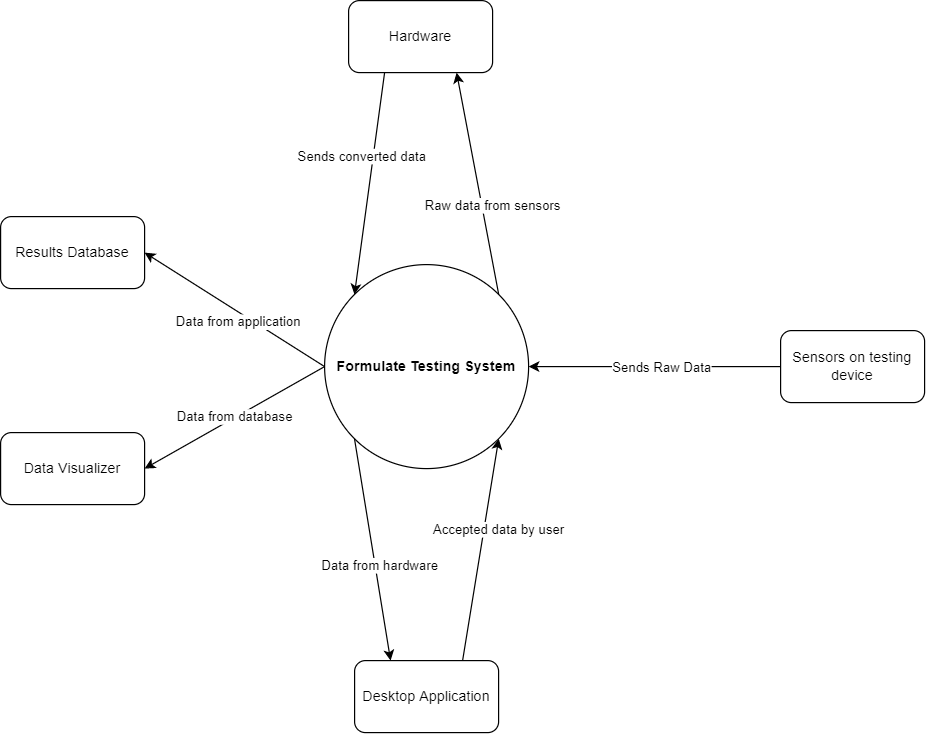
\includegraphics[width=1.1\textwidth]{sys_context_diagram}
  \caption{Formulate Context Diagram}
  \end{center}
  \end{figure}
  \newpage

\section{Project Overview}

\subsection{Normal Behaviour}
During normal operation the device should work as follows, the user has an option to either connect wired or wirelessly to our device, regardless of which method they choose the results will be consistent between the two. To connect to the device the user will open our desktop application and either create an account or log in to an existing account, this will lead them to the home page where the user will select the connection method as wireless or wired.\\

Before the user can start any testing they will need to secure our device on a vehicle they are testing. Our device has 2 methods of mounting, either the hose clamp holes can be used or the custom mount. After the device is secure the user will need to ensure that all the correct sensors are attached. To conduct any testing the user will first fill out the test parameters of the specific test they are conducting and they will also upload pictures of the current configuration of the car. The user will then go to the test page in our application and start the test, during testing our hardware will collect the sensor data and send it to the PC. When the user stops the test they will be able to preview all the raw data collected from the test and either declines the data or send it to the database. When the user sends data to the database all the sensor data will be sent along with the test parameters and pictures.\\

If the user wants to view previous test data they will be able to, using a Power Bi dashboard, this dashboard will read all the data from the database and display it to the user in a more presentable way. The Power Bi dashboard will allow the user to do comparisons between tests and take a quick glance if the tests they conducted passed all the required tests.

\begin{figure}[h!]
  \begin{center}
  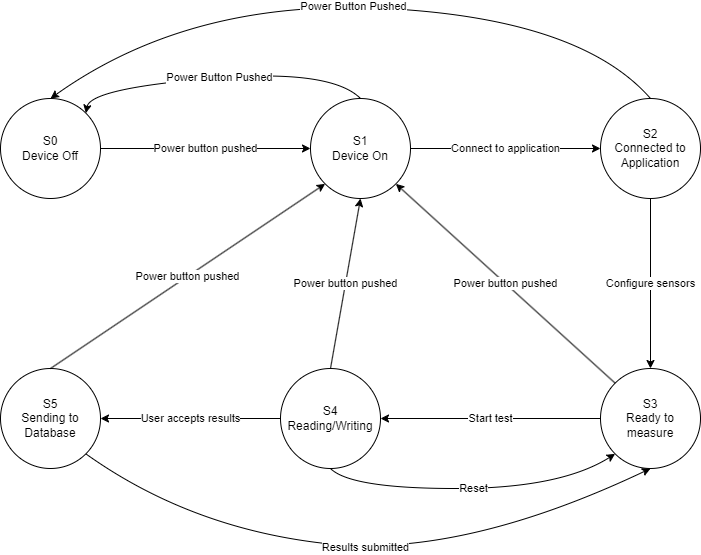
\includegraphics[width=0.5\textwidth]{state_machine_diagram.png}
  \caption{Finite State Machine}
  \end{center}
  \end{figure}
  \newpage

\subsection{Undesired Event Handling}
There might be cases where undesired events occur and to minimize any issues caused to the user we tried to account for them
\subsubsection{Loss of Power/Connection}
If at any point the connection between the PC and the device fails, i.e the power goes out or the device gets unplugged, we have implemented a backup system to ensure that no testing data is lost. Whenever data is sent to the PC it is also simultaneously sent to the local storage on the device itself. The onboard MicroSD Card will have all the data saved and the user will be able to recover it if anything were to go wrong.

\subsubsection{Excessive Vibration/Shaking}
Since our device will be in an environment where there might be lots of vibration we decided to create a custom PCB instead of using normal jumper cables and a breadboard. This ensures that regardless of the amount of motion the connections between the components inside our device will be fixed.

\subsubsection{Loss of Data Packets}
When data from our device is being sent to the PC there might be situations where some data is lost or the entire string of data is not sent correctly. To make sure that we are only reading data from complete bytestrings each bytestring start with 'B' and ends with 'E' and our python program checks to make sure that the data we are saving has both those values.

\wss{How you will approach undesired events}

\newpage
\subsection{Component Diagram}
\begin{figure}[hbt!]
  \begin{center}
  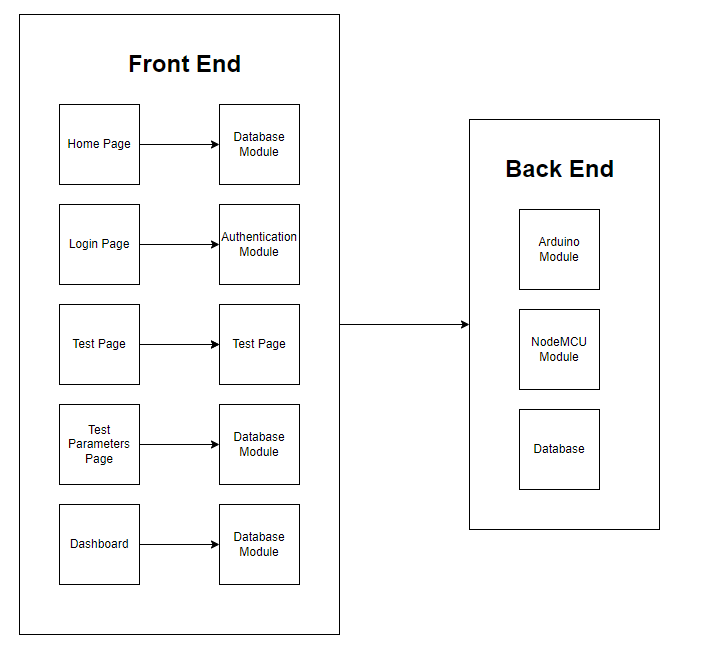
\includegraphics[width=0.7\textwidth]{component_diagram.png}
  \caption{Component Diagram} 
  \end{center}
  \end{figure}

\newpage
\subsection{Connection Between Requirements and Design} \label{SecConnection}
The following requirements are from the SRS document.

\begin{itemize}
  \item[FR1,FR5:] To measure vibration we chose to use an accelerometer that outputs in units of G's. For temperature, we are using an LM35 temperature sensor which provides temperature in celsius and has an accuracy of +- 1 degree. To measure humidity we are using a DHT11 sensor which gives us the relative humidity in percent. The accelerometer also provides shock data which just needs some post-processing
  \item[FR2:] The device transmits data using the UART protocol to the PC when it is connected via a wire.
  \item[FR3,FR4:] The device will have the start and stop buttons to control the tests inside the desktop application so the user can conduct tests remotely.
  \item[FR6:] The user can preview the data after a test once they stop the test. A table will populate with all the raw data from the test on the testing page of the desktop application
  \item[FR7:] After the user previews the test they will be able to decline or submit the test to our database. The table of test values will be sent to our Azure database once the user approves.
  \item[FR8:] The Power Bi dashboard will connect to the Azure database and will be able to read all the test data
  \item[FR9:] The device will be clamped down to a ClickBond mount
  \item[FR11:] Our device is going to contain 4 AA batteries to power the entire thing, this allows for the user to be able to quickly swap out old batteries for new ones if they die.
  \item[FR12:] Using an ESP8266 our device will wirelessly communicate with our desktop application through Wi-Fi and will be using TCP to send data back and forth.
  \item[FR16:]  The device has an onboard programming mode switch which will allow users to change setting on the ESP8266 or the Arduino
  \item[FR17:] The device will have a terminal block which will allow users to connect to 6 digital ports and 6 analog ports      
  
\end{itemize}

\wss{The intention of this section is to document decisions that are made
  ``between'' the requirements and the design.  To satisfy some requirements,
  design decisions need to be made.  Rather than make these decisions implicit,
  they are explicitly recorded here.  For instance, if a program has security
  requirements, a specific design decision may be made to satisfy those
  requirements with a password.}


\newpage
\section{System Variables}

\wss{Include this section for Mechatronics projects}

\subsection{Monitored Variables}
  \begin{table}[!h]
  \begin{tabular}{| p{0.23\textwidth} | p{0.10\textwidth}| p{0.10\textwidth}| p{0.46\textwidth}|}
    \hline
    \rowcolor[gray]{0.9}
    Monitored Variable & Type & Units & Description\\
    \hline
    m\_vibration & Analog& V& A signal monitoring the vibration resistance of the motor \\
    \hline
    m\_humidity & Analog & V & A signal monitoring the humidity of the motor’s environment \\
    \hline
    m\_temperature & Analog & V & A signal monitoring the temperature of the motor’s environment \\
    \hline
    m\_shock & Analog & V & A signal monitoring the shock resistance of the motor \\
    \hline
    m\_conv\_vibration & Digital & g  & Converted vibration values that are in useful units \\
    \hline
    m\_conv\_humidity & Digital & \% & Converted humidity values that are in useful units \\
    \hline
    m\_conv\_temperature & Digital & \textdegree C & Converted temperature values that are in useful units \\
    \hline
    m\_conv\_shock & Digital & g & Converted shock values that are in useful units \\
    \hline
    m\_data\_accepted & Digital & T/F & Determines if user has accepted the results and wants to send it to the database \\
    \hline
  \end{tabular}
  \caption{Monitored Variables}
  \end{table}

\subsection{Controlled Variables}
  \begin{table}[!h]
  \begin{tabular}{| p{0.23\textwidth} | p{0.10\textwidth}| p{0.10\textwidth}| p{0.46\textwidth}|}
    \hline
    \rowcolor[gray]{0.9}
    Controlled Variable & Type & Units & Description\\
    \hline
    c\_green\_light& Digital& 1/0& Green LED light on testing device that indicates passed measurements \\
    \hline
    c\_red\_light& Digital & 1/0 & Red LED light on testing device that indicates failed measurements \\
    \hline
    c\_sent\_to\_database & Digital & T/F & Determines if results displayed on the application are sent to the database \\
    \hline
  \end{tabular}
  \caption{Controlled Variables}
  \end{table}

\subsection{Constants Variables}
  \begin{table}[!h]
  \begin{tabular}{| p{0.23\textwidth} | p{0.10\textwidth}| p{0.10\textwidth}| p{0.46\textwidth}|}
    \hline
    \rowcolor[gray]{0.9}
    Constant & Units & Value & Description\\
    \hline
    k\_temperature\_range& \textdegree C& 5-40& Acceptable ambient temperature values for a Formula Electric motor \\
    \hline
    k\_humidity\_range& \% & 5-85 & Acceptable relative humidity values for a Formula electric motor \\
    \hline
    k\_max\_shock & g & 100 & Maximum shock resistance for a Formula Electric motor \\
    \hline
    k\_max\_vibration & g & 20 & Maximum vibration resistance for a Formula Electric motor \\
    \hline
  \end{tabular}
  \caption{Constants Variables}
  \end{table}

\section{User Interfaces}

\subsection{Desktop Application}
The user interface for the desktop application is designed through Qt designer, a software for designing and building GUIs through the Qt library. Qt designer generates UI files which can be converted to python scripts that build the static design and layout of the GUI. The desktop application is essentially multiple pages stacked on each other that change based on which buttons are clicked. The GUI is comprised of a left bar menu, top bar, and content pages being in the center, refer to figure 1 and 2 in the Appendix. Navigation through the application is done using the sidebar menu, where users can toggle the full menu and press on which page they want to go. The top bar will be used for extra functionality such as accessing user details, minimizing screen, etc. Users interact with the application using buttons to perform a variety of functions and form fields in which they can enter test/user information.

\subsection{Hardware}
The user will interface with the hardware as follows, they will mount a sensor to the top of our device and connect it via a terminal block which is on the side of the device. The device will then be mounted to the Formula vehicle and the rest of the operations will take place on the Desktop Application.

\subsection{Web Dashboard}
The user interface for the dashboard will allow the user to visualize data received from the database through a dashboard using Power Bi. After a test is conducted the user will be able to view the data on the Power Bi website. It will prompt the user to view the data in a variety of graphs and tables which will allow the user to interpret the data in more manageable and understandable way. The design is made with user in mind allowing them to find and view the data in the dashboard in a variety of ways since different types of data will be stored in the database.



\wss{Design of user interface for software and hardware.  Attach an appendix if
needed. Drawings, Sketches, Figma}

\section{Design of Hardware}

The hardware for our project will include a 3D-printed chassis that will house all our electrical components. Our chassis was designed to meet the requirements outlined in our SRS document. The main requirement our chassis needs to meet is how easily it mounts to the Formula E car. We are currently implementing 2 methods of mounting the device onto the car, the first method consists of attaching a ClickBond mount to the base of the car, and our device will have a mechanism that connects to the mount. The second method is for attaching the device to any other surface of the vehicle, our chassis has slots at the bottom through which hose clamps can fit to allow the device to be clamped to any surface. A preliminary design can be found in Figure 6.

\wss{Most relevant for mechatronics projects}
\wss{Show what will be acquired}
\wss{Show what will be built, with detail on fabrication and materials}
\wss{Include appendices as appropriate, possibly with sketches, drawings, CAD, etc}

\newpage
\section{Design of Electrical Components}

\wss{Most relevant for mechatronics projects}
\wss{Show what will be acquired}
\wss{Show what will be built, with detail on fabrication and materials}
\wss{Include appendices as appropriate, possibly with sketches, drawings,
circuit diagrams, etc}

The electrical components were selected to address the functional requirements regarding robust sensor connection points, wireless functionality, and backup data collection capabilities. These capabilities were enabled using hardware modules selected to interface with the embedded device. \\

The Arduino Uno R3 (Uno) was the choice electrical component for the device's microcontroller. While other microcontrollers on the market were also capable of flexibly collecting data from a multitude of sensors, the Uno stood out as the optimal choice because of low monetary cost in hardware and the relatively high accessibility at large e-commerce platforms for the Formula Electric Team to purchase. In addition, the likelihood of the Formula Electric team using parts of the testing budget on the microcontroller was minimized as many Formula Electric members already posessed an Uno board. \\

To support testing application flexibility in cases where no direct connections to power were available, four 1.5 volt batteries with a battery holder was used to provide the Uno with adequate power for on vehicle testing sessions. \\

A single pole, double throw (SPDT) power switch was used to quickly connect and disconnect the four 1.5 volt batteries with the circuit connecting all electrical components. The switch was oriented such that the common pin actuated to connect either the 9V battery to the circuit or the circuit directly to ground. \\

Although the Uno provided many functionalities, the standard Uno model did not natively support wireless communication capabilities. As a result, the group chose to integrate a hardware module capable of a Transmission Control Protocol / Internet Protocol (TCP/IP) stack through an ESP8266 Software On Chip (SOC). The electrical component containing the ESP8266 SOC that was selected was the Node MCU 1.0. The Node MCU 1.0 is a development board with the ESP8266 SOC already built onto the Node MCU's PCB in addition to an on-board voltage regulator for the development board's 3.3 volt input power requirement. \\

A single pole, single throw (SPST) switch packaged with four ports was also required to interface the Node MCU 1.0 module with the Uno during initial device comissioning. Specifically, three of the four ports were used to disconnect the 3.3 volt power, transmit (TX), and recieve (RX) signal between the wifi module and the microcontroller when flashing the wifi module with firmware via a micro Universal Serial Bus (USB) port. When the one time firmware flash is complete, the three switches could be actuated to reconnect the power and signal connections between the two components. Despite the connect/disconnect functionality requiring only three of the four ports, a four port SPST switch was selected due to the high accesibility on large electronics e-commerce platforms relative to three port SPST switches. \\

Two diagnostic light-emitting diode's (LED) were used to provide the user with feedback on the live transmission status of the wifi module. The first diagnostic signal conveyed when a connection between the wifi module and the desktop application was established, showing the module was capable of transmitting data. This required the first LED to visually depict the active signal to the user. The second diagnostic signal conveyed when the wifi module was actively transmitting data live to the desktop application. This required the second LED to visually depict the active signal to the user. \\

Two resistors were also paired with the diagnostic LED's to primarily limit the current going through each LED, but also the luminosity of both LED's. Limiting the current through each LED was an important consideration as it supports a consistent luminoscity in the LED's and mitigates premature breakdown of the LED due to a high current burnout. \\

Backup data storage to local memory in the event of wireless communication error due to the wifi module's failure or device operation outside the wifi router's range necessitated the use of a local memory storage electrical component. A 32 GigaByte (GB) micro Secure Digital (SD) card paired with a micro SD card adapter was used to provide the Uno with local memory storage to concurrently write test data to the SD card while also sending data over wifi to the desktop application. SanDisk, the microSD card manufacturer, was chosen primarily due to their cost effectiveness against other microSD manufacturers as measured by GB/dollar. Similarly, Geek Story was used as the microSD card adapter manufacturer as a result of their cost-effectiveness. \\

Robust sensor connection components between the sensor and the Uno's input ports were required for tests in physically demanding scenario's as loose or broken connections from high vibration or shock compromised the reliability of the sensor readings and thus the test data. As a result, Phoenix Contact's through hole, 8 port terminal blocks were used because the terminal block style connections provided a stronger connective interface between the sensor conductors and the Uno's ports. \\

Robust connections between all components of the circuit such as the electrical connections between the Uno, wifi module, micro SD card adapter, switches, and LED's also required a more robust solution relative to jumper wires. As a result, the group chose to design and manufacture a Printed Circuit Board (PCB) onto which all electrical components outlined could be soldered onto the board for a higher strength connection. \\
\newpage

The required electrical connections between the micro SD adapters pinouts and the Uno's pinouts were first outlined to organize the connection layout in the table below. \\

\begin{table}[H]
  \centering
  \begin{tabular}{|p{2cm}|p{6cm}|p{2cm}|p{2cm}|}
  \hline
  \rowcolor[gray]{0.9}
  \multicolumn{1}{|c|}{\textbf{Pin Name}} & \multicolumn{1}{c|}{\textbf{Pin Description}} & \multicolumn{1}{|c|}{\textbf{Arduino Port}} & \multicolumn{1}{|c|}{\textbf{Arduino Port Description}} 
  \\ \hline
  VCC
  & 5 Volt
  & 5 Volt
  & Power output
  \newline                                
  \\ \hline

  GND                              
  & Ground
  & Ground
  & Ground
  \newline                                
  \\ \hline

  MISO                          
  & SPI output from microSD
  & 12
  & Digital I/O
  \newline                                
  \\ \hline

  MOSI                                
  & SPI input to microSD
  & 11 
  & Digital I/O
  \newline                            
  \\ \hline

  SCK                                
  & Synchronize data transmission via Arduino clock
  & 13 
  & Digital I/O
  \newline                            
  \\ \hline

  CS                                
  & Select slave device on SPI bus
  & 10 
  & Digital I/O
  \newline                            
  \\ \hline

  \end{tabular}
  \caption{MicroSD Adapter to Uno Pinout}
\end{table}


The required electrical connections between the wifi module's pinouts and the Uno's pinouts were also outlined to organize the connection layout in the table below. \\

\begin{table}[H]
  \centering
  \begin{tabular}{|p{2cm}|p{6cm}|p{2cm}|p{2cm}|}
  \hline
  \rowcolor[gray]{0.9}
  \multicolumn{1}{|c|}{\textbf{Pin Name}} & \multicolumn{1}{c|}{\textbf{Pin Description}} & \multicolumn{1}{|c|}{\textbf{Arduino Port}} & \multicolumn{1}{|c|}{\textbf{Arduino Port Description}} 
  \\ \hline
  3V3
  & 3.3 Volt
  & 3.3 Volt
  & Power output
  \newline                                
  \\ \hline

  GND                              
  & Ground
  & Ground
  & Ground
  \newline                                
  \\ \hline

  TX                          
  & Transmit
  & 2
  & Digital I/O
  \newline                                
  \\ \hline

  RX                                
  & Recieve
  & 3
  & Digital I/O
  \newline                            
  \\ \hline


  \end{tabular}
  \caption{Wi-Fi Module to Uno Pinout}
\end{table}


\newpage

A final list of the required electrical components was shown below. \\

\begin{table}[H]
  \centering
  \begin{tabular}{|p{3cm}|p{2cm}|p{4cm}|p{4cm}|p{2cm}|}
  \hline
  \rowcolor[gray]{0.9}
  \multicolumn{1}{|c|}{\textbf{Component}} & \multicolumn{1}{c|}{\textbf{Manufacturer}} & \multicolumn{1}{c|}{\textbf{Part Number}} & \multicolumn{1}{c|}{\textbf{Description}} & \multicolumn{1}{|c|}{\textbf{Quantity}}
  \\ \hline
  Microcontroller
  & Arduino
  & Uno R3
  & System micro-controller
  & 1
  \newline                                
  \\ \hline

  Wifi Module                              
  & NodeMCU
  & 1.0
  & System wifi 
  & 1
  \newline                                
  \\ \hline

  Micro SD Adapter                          
  & Geek Story
  & N/A
  & Local memory interface
  & 1
  \newline                                
  \\ \hline

  Micro SD Card                                
  & Sandisk
  & SDSQUAR-032G-GN6MA
  & System local memory
  & 1
  \newline                            
  \\ \hline

  Battery                                
  & Duracell
  & 4330206640
  & System power
  & 4
  \newline                            
  \\ \hline

  SPDT Switch                                
  & E-Switch
  & 100SPTITI1B4M2QE
  & System power switch
  & 1
  \newline                            
  \\ \hline

  4 Port SPST Switch                                
  & TE
  & 435640-2
  & Wifi signal control switch
  & 1
  \newline                            
  \\ \hline

  Through Hole Terminal Block                                
  & Phoenix Contact
  & 1715789
  & System sensor ports
  & 2
  \newline                            
  \\ \hline

  LED                                
  & Kingbright
  & WP7113ID5V
  & LED Resistor
  & 2
  \newline                            
  \\ \hline

  Resistor                                
  & TE
  & CBT25J100R
  & LED Resistor
  & 2
  \newline                            
  \\ \hline

  Custom PCB                                
  & JLCPCB
  & N/A
  & System PCB
  & 1
  \newline                            
  \\ \hline

  \end{tabular}
  \caption{Component List}
\end{table}

The electrical schematic for the overall circuit containing all components was designed in Kicad and was shown in Appendix C. The PCB layout was also designed in Kicad and was shown in Appendix C. The PCB layout was then fabricated by the manufacturer JLCPCB. \\

\newpage





\newpage
\section{Design of Communication Protocols}
Our project mainly uses two ways to communicate. The user will either directly plug the device into their computer or they will wirelessly communicate with the device over Wi-Fi. Each of the sensors that are connected to the Arduino uses different protocols to send data.


\begin{table}[!h]
\begin{tabular}{| p{0.50\textwidth} | p{0.30\textwidth}|}
  \hline
  \rowcolor[gray]{0.9}
  Device & Communication Protocol \\
  \hline
  MicroSD Card Module & SPI\\
  \hline
  Accelerometer (ADXL345) &  I2C\\
  \hline
  Temperature Sensor (L535) & Single Bus \\
  \hline
  Humidity Sensor (DHT11) & Single Bus \\
  \hline
  Wi-Fi Module (ESP8266, NodeMCU 1.0) & UART \\
  \hline
 
\end{tabular}
\caption{Communication Protocols}
\end{table}




To simplify the communication protocol, after the Arduino reads all the values from the sensors it formats them into bytestring to send to either the Wi-Fi module or the PC directly via USB. The bytestring takes the form

\begin{verbatim}
B<X-VAL>S<Y-VAL>S<Z-VAL>S<TEMP-VAL>S<HUMIDITY-VAL>E
\end{verbatim}

The order in which sensor values are sent are the following order; Vibration in X, Vibration in Y, Vibration in Z, Temperature, and Humidity. Each bytestring starts with 'B' and ends with 'E', after the data is sent to the PC our python program parses through the received bytestring and only stores values from complete bytestrings, it checks for the 'B' and the 'E'.Each of the values in the bytestring is separated with 'S', our python program is then able to split the bytestring and read the correct information from it. When the device is directly plugged into the PC it sends the data over USB via serial and data is sent every second. The other way of receiving data is over Wi-Fi, the Arduino takes the bytestring and sends it using the TX and RX pins to the NodeMCU which then relays the information to the PC via a TCP connection.\\

To connect the device to our PC wirelessly there are two main methods we have implemented. The first method is to make our device act as an access point, this means the PC will directly connect to the device and they will exchange information via a TCP connection. The second method would be to connect our device to a central hub and also connect our PC to the same hub, this would require an ethernet connection to be present to plug the hub in. Using both methods our ESP8266 acts as a relay device that passes the information from the Arduino to the PC via TCP.


\wss{If appropriate}
\newpage
\section{Timeline}

\begin{table}[!h]
  \begin{tabular}{| p{0.30\textwidth} | p{0.30\textwidth}| p{0.30\textwidth}|}
    \hline
    \rowcolor[gray]{0.9}
    Objective & Deadline & Assigned Member\\
    \hline
    Device mounting mechanism design & 2023/01/28 & Ahmed\\
    \hline
    Sensor mounting mechanism design &  2023/01/23 & Tioluwalayomi\\
    \hline
    3D chassis print & 2023/01/29 & Stephen \\
    \hline
    Test and validate PCB & 2023/01/22 & Muhanad \\
    \hline
    Assemble circuit on PCB & 2023/01/24 & Ahmed \\
    \hline
    Modularize Arduino code for hardware interface & 2023/01/22 & Tioluwalayomi \\
    \hline
    Finalize dashboard design & 2023/02/06 & Tioluwalayomi \\
    \hline
    Finalize home page & 2023/02/06 & Muhanad \\
    \hline
    Finalize test parameter page & 2023/02/06 & Ahmed\\
    \hline
    Finalize test page & 2023/02/06 & Tioluwalayomi\\
    \hline
    Finalize login page & 2023/02/06 & Stephen\\
    \hline
   
  \end{tabular}
  \caption{Timeline}
\end{table}

\wss{Schedule of tasks and who is responsible}

% \bibliographystyle {plainnat}
% \bibliography{../../../refs/References}

\newpage{}

\appendix

\section{Interface}
\begin{figure}[h!]
  \begin{center}
  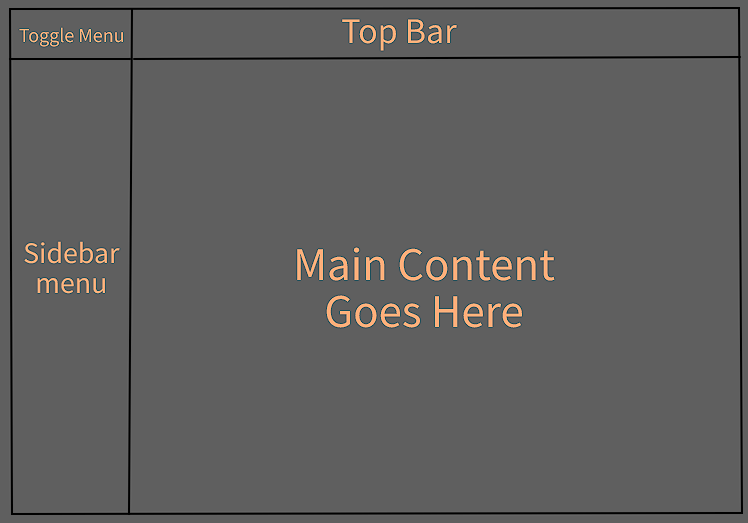
\includegraphics[width=0.7\textwidth]{GUI_sketch}
  \caption{Basic layout of GUI}
  \label{Fig_SystemContext} 
  \end{center}
  \end{figure}

\begin{figure}[hbt!]
  \begin{center}
  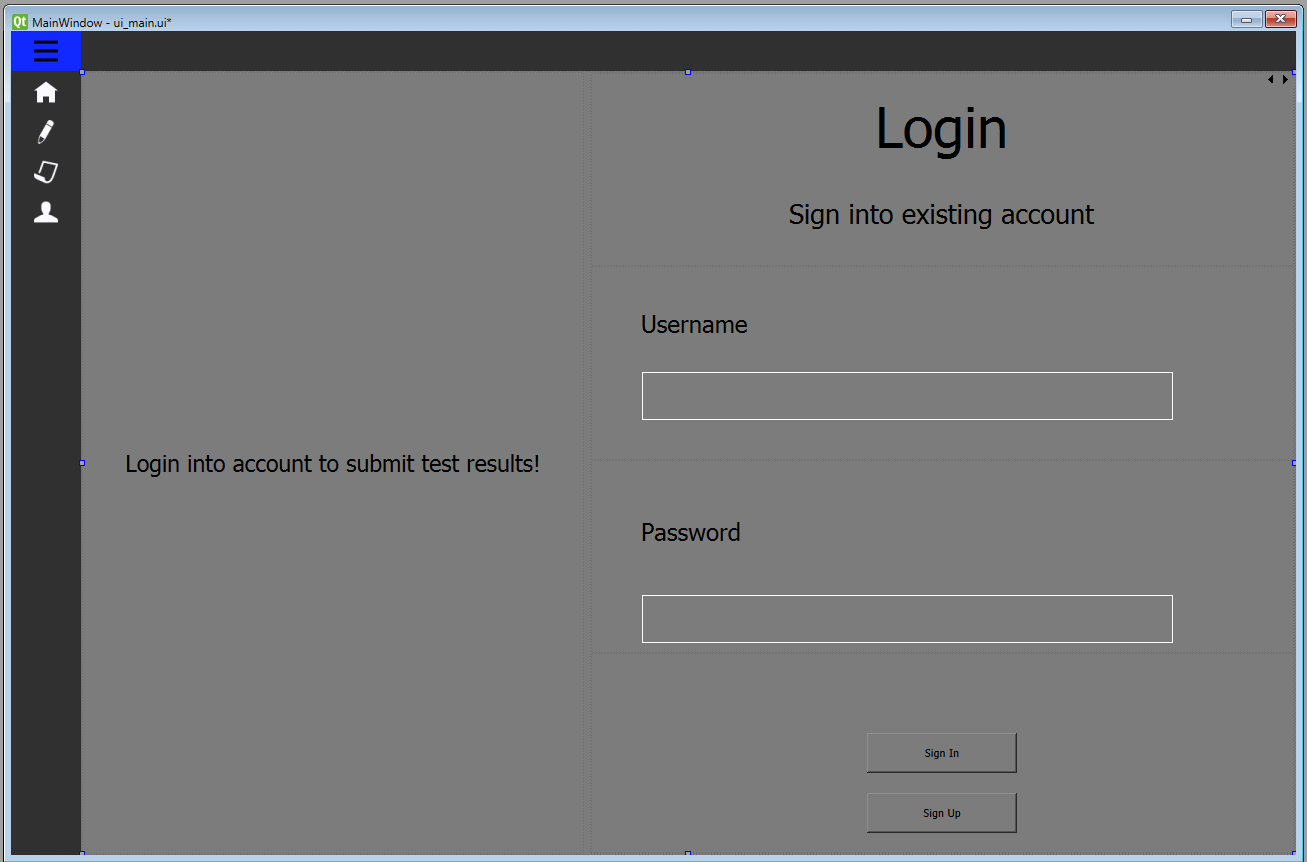
\includegraphics[width=0.7\textwidth]{GUI_designer}
  \caption{GUI design in Qt Designer}
  \label{Fig_SystemContext} 
  \end{center}
  \end{figure}

\wss{Include additional information related to the appearance of, and
interaction with, the user interface}

\section{Mechanical Hardware}
  \begin{figure}[h!]
    \begin{center}
    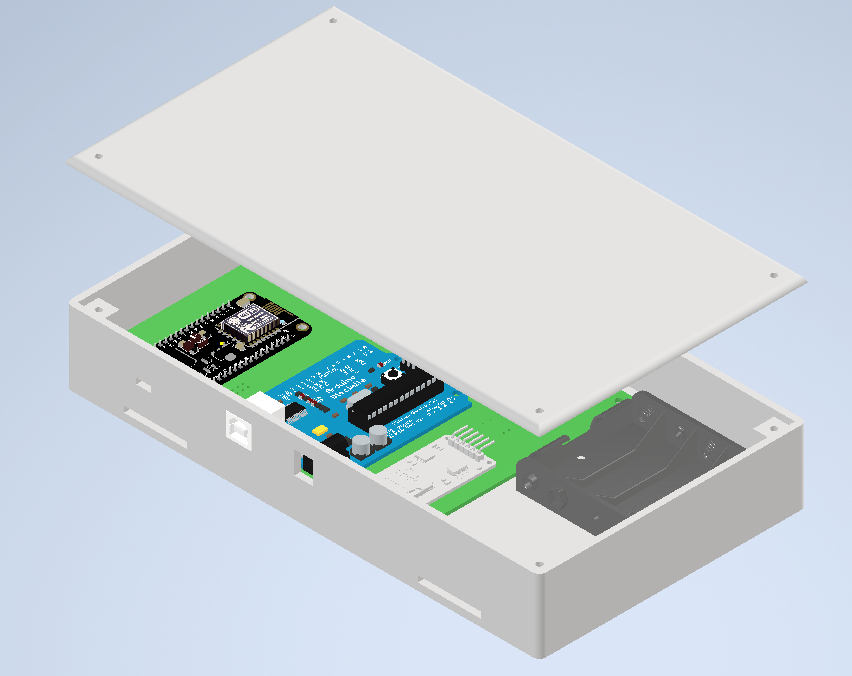
\includegraphics[width=0.6\textwidth]{Chassis_3D_Render.png}
    \caption{Chassis 3D Render}
    \label{Fig_SystemContext} 
    \end{center}
    \end{figure}

  \begin{figure}[h!]
    \begin{center}
    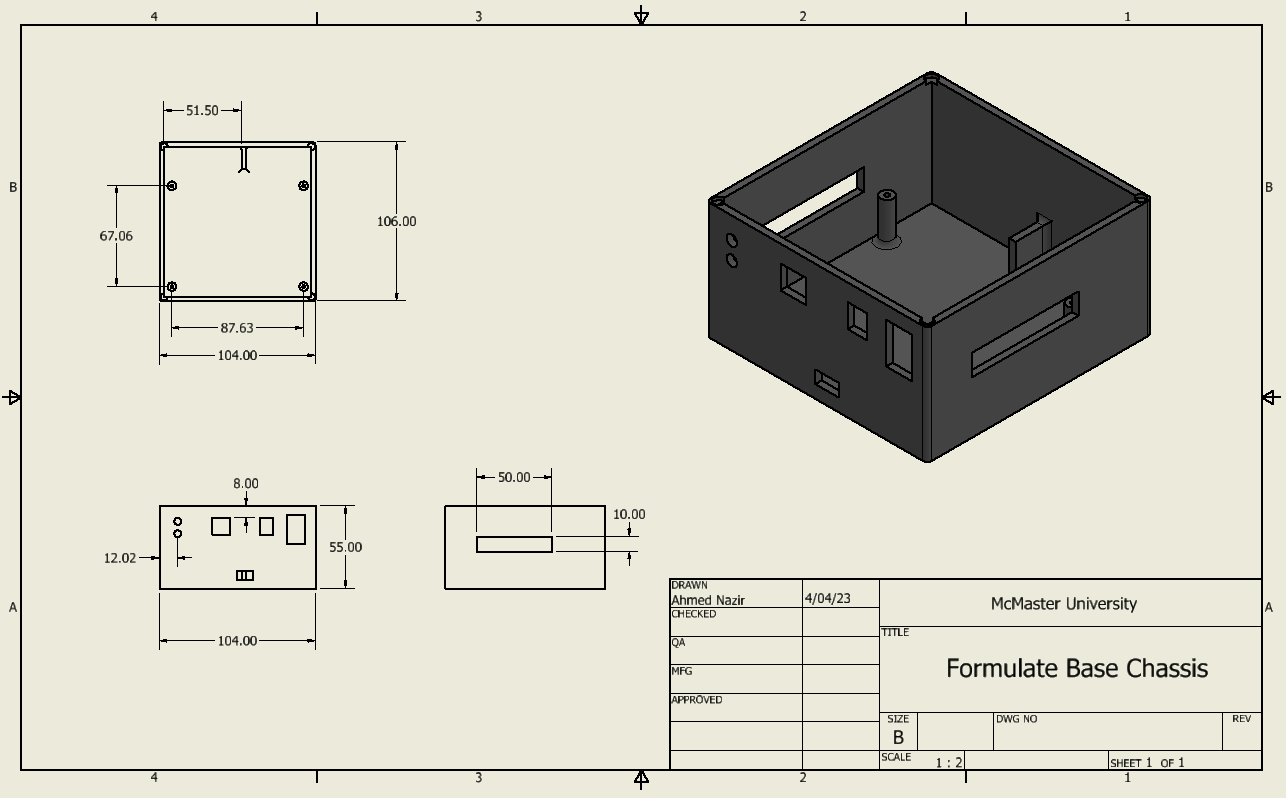
\includegraphics[width=0.7\textwidth]{Chassis_Drawing.png}
    \caption{Chassis Drawing}
    \label{Fig_SystemContext} 
    \end{center}
    \end{figure}


\newpage
\section{Electrical Components}

\subsection{Electrical Schematic}
\begin{figure}[h!]
  \begin{center}
  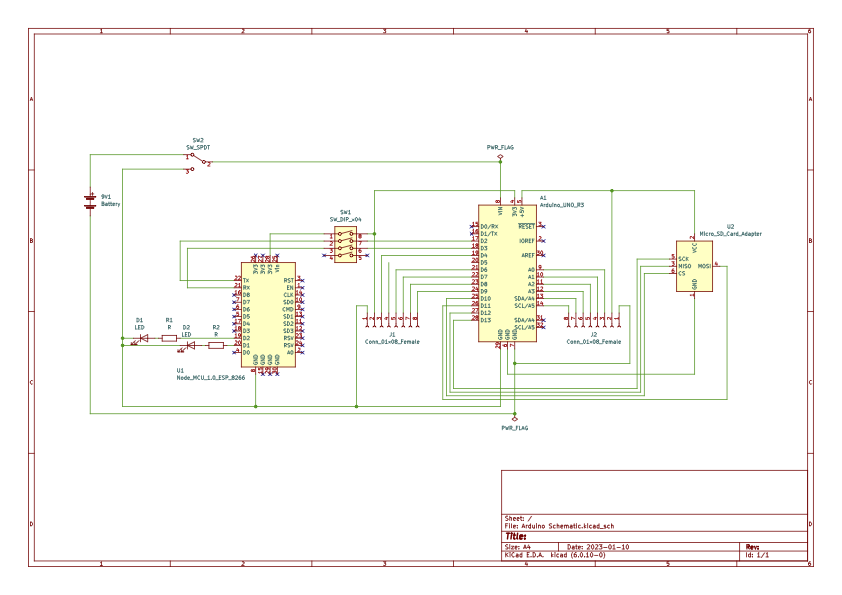
\includegraphics[width=1.0\textwidth]{Electrical_Schematic}
  \caption{Electrical Schematic in Kicad}
  \end{center}
  \end{figure}
  \newpage

\subsection{PCB Layout}
\begin{figure}[h!]
  \begin{center}
  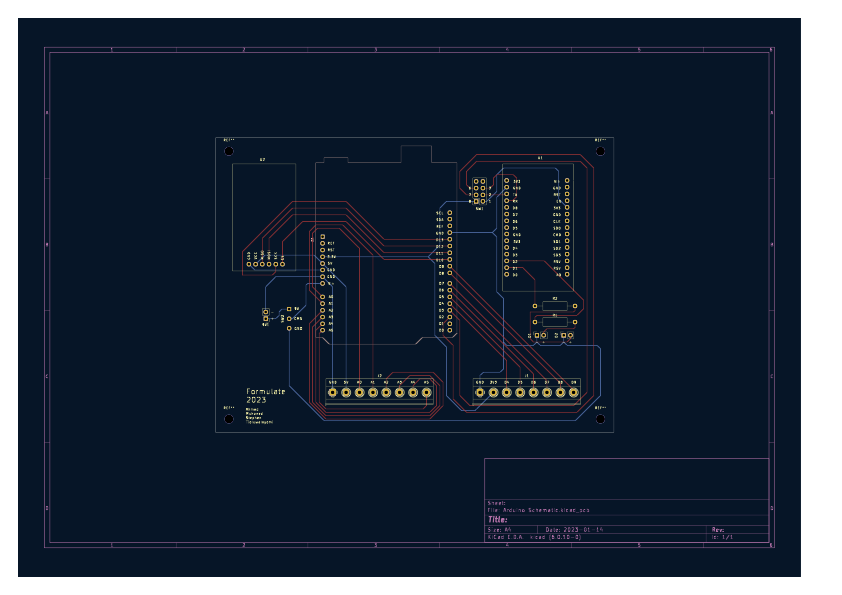
\includegraphics[width=1.0\textwidth]{PCB_Schematic}
  \caption{PCB Layout in Kicad}
  \end{center}
  \end{figure}
  \newpage

\subsection{PCB CAD}
\begin{figure}[h!]
  \begin{center}
  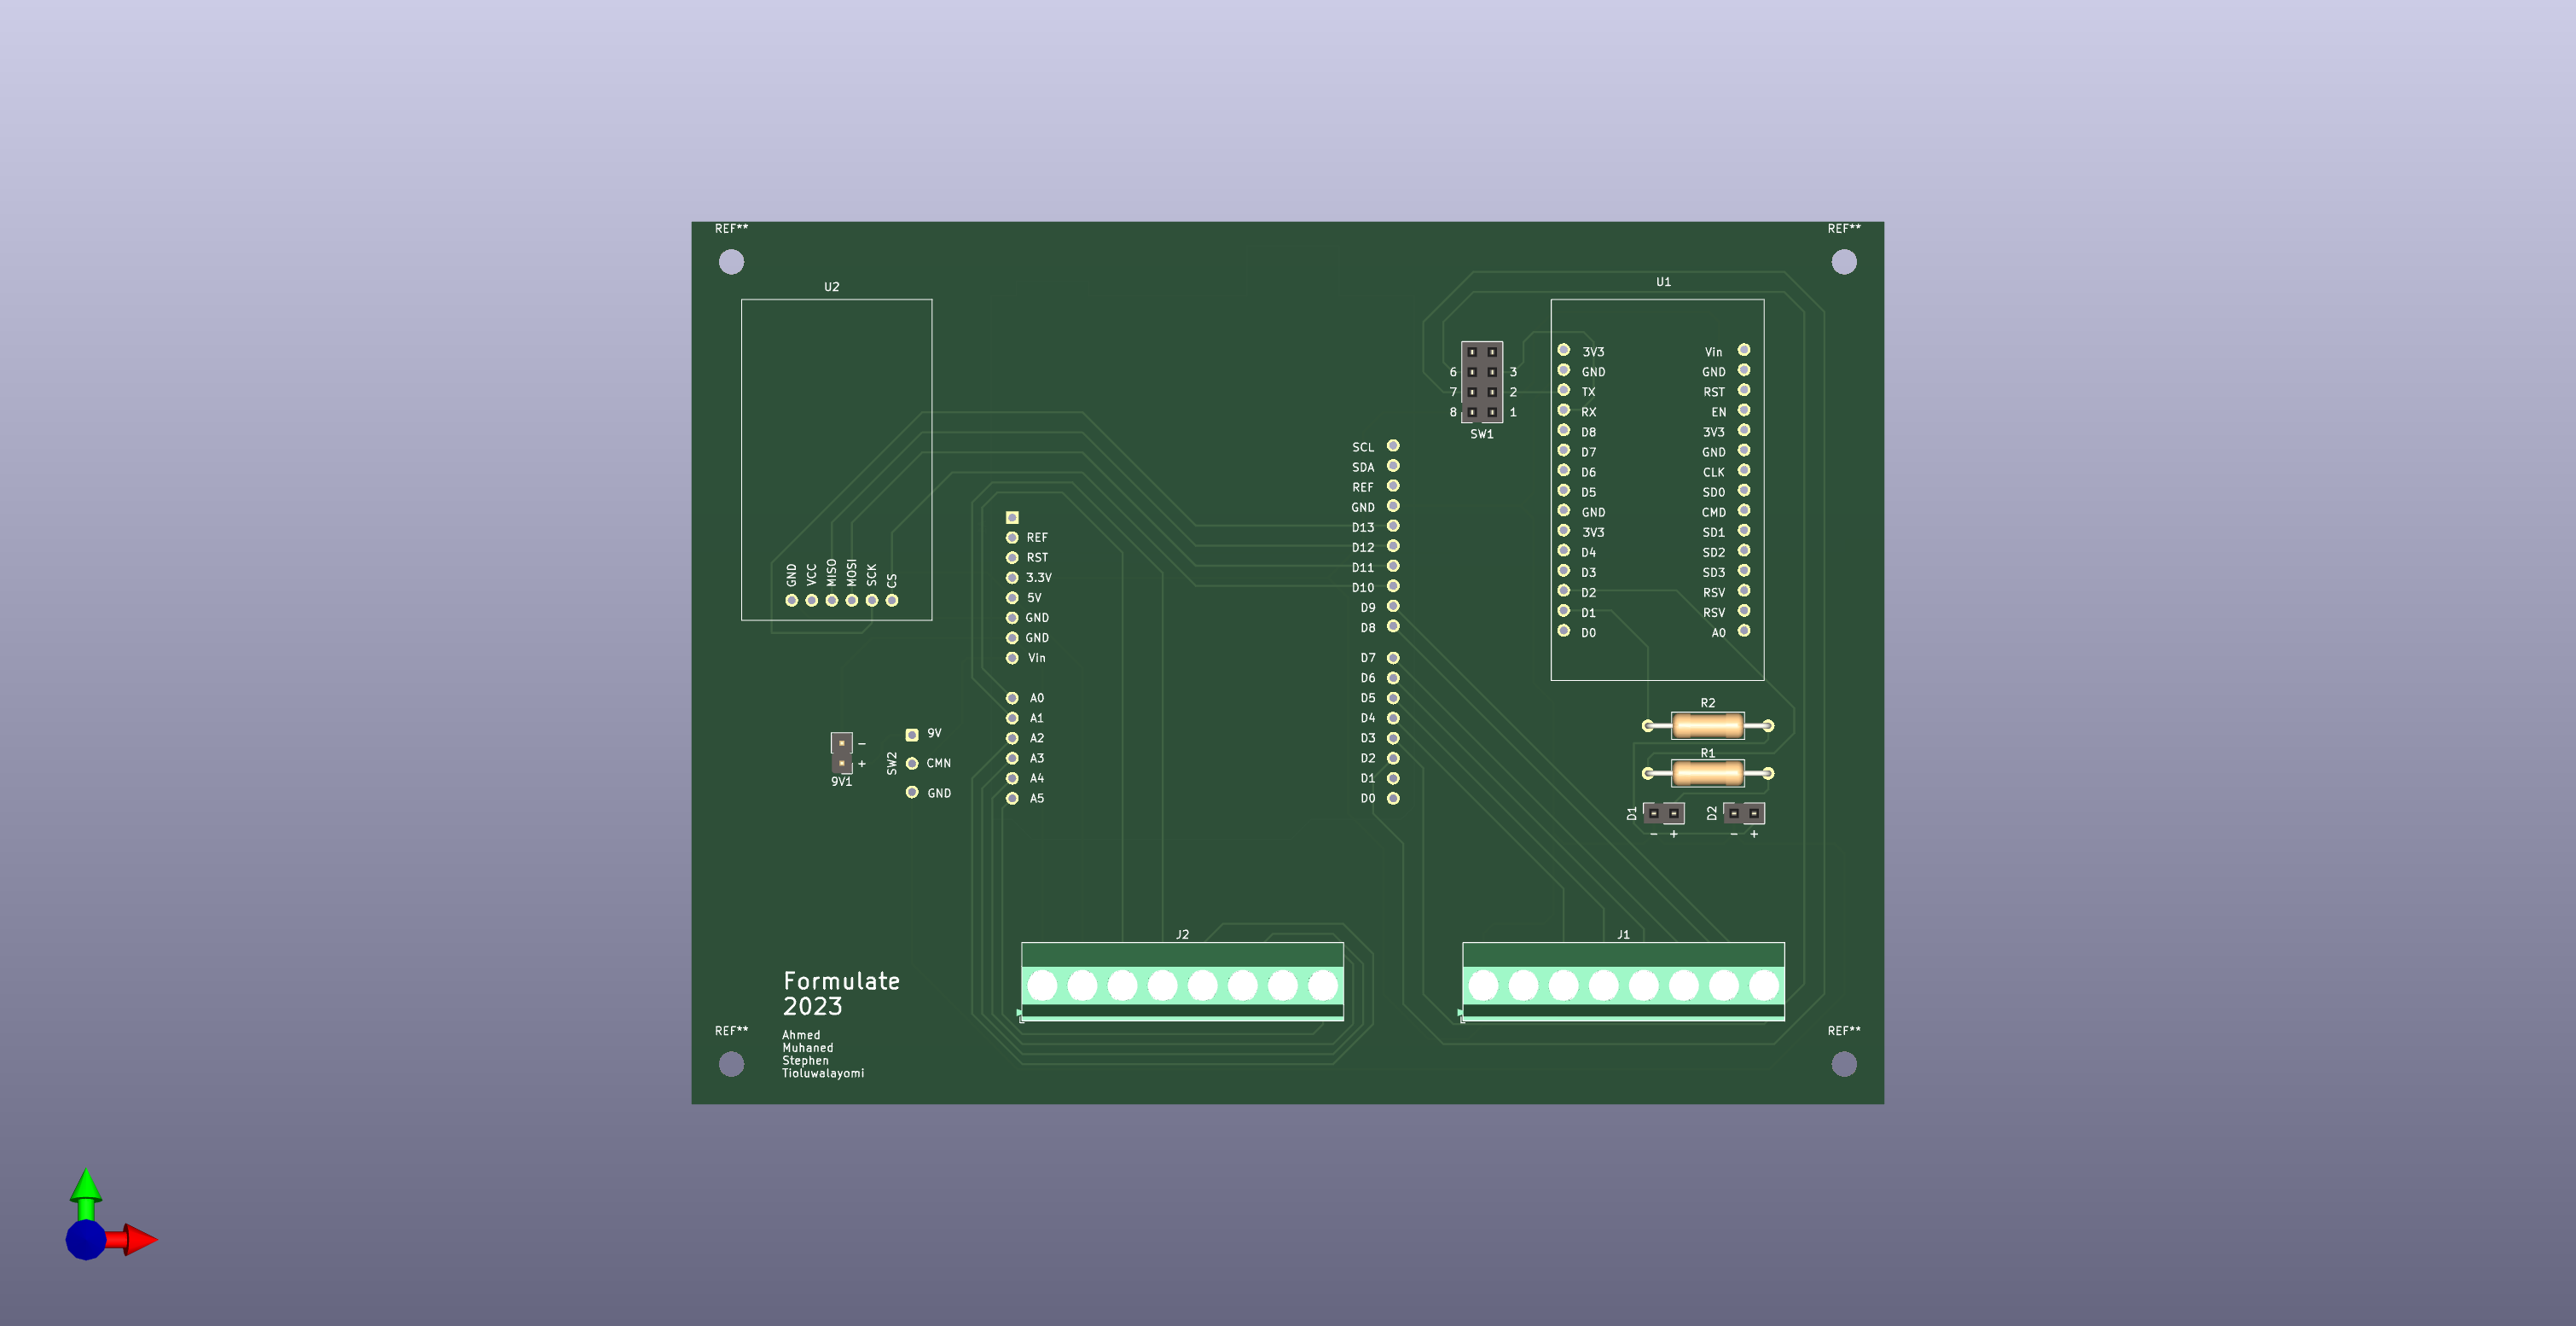
\includegraphics[width=1.0\textwidth]{PCB_Front_View}
  \caption{Top view of the PCB}
  \end{center}
  \end{figure}
  \newpage

\subsection{PCB CAD}
\begin{figure}[h!]
  \begin{center}
  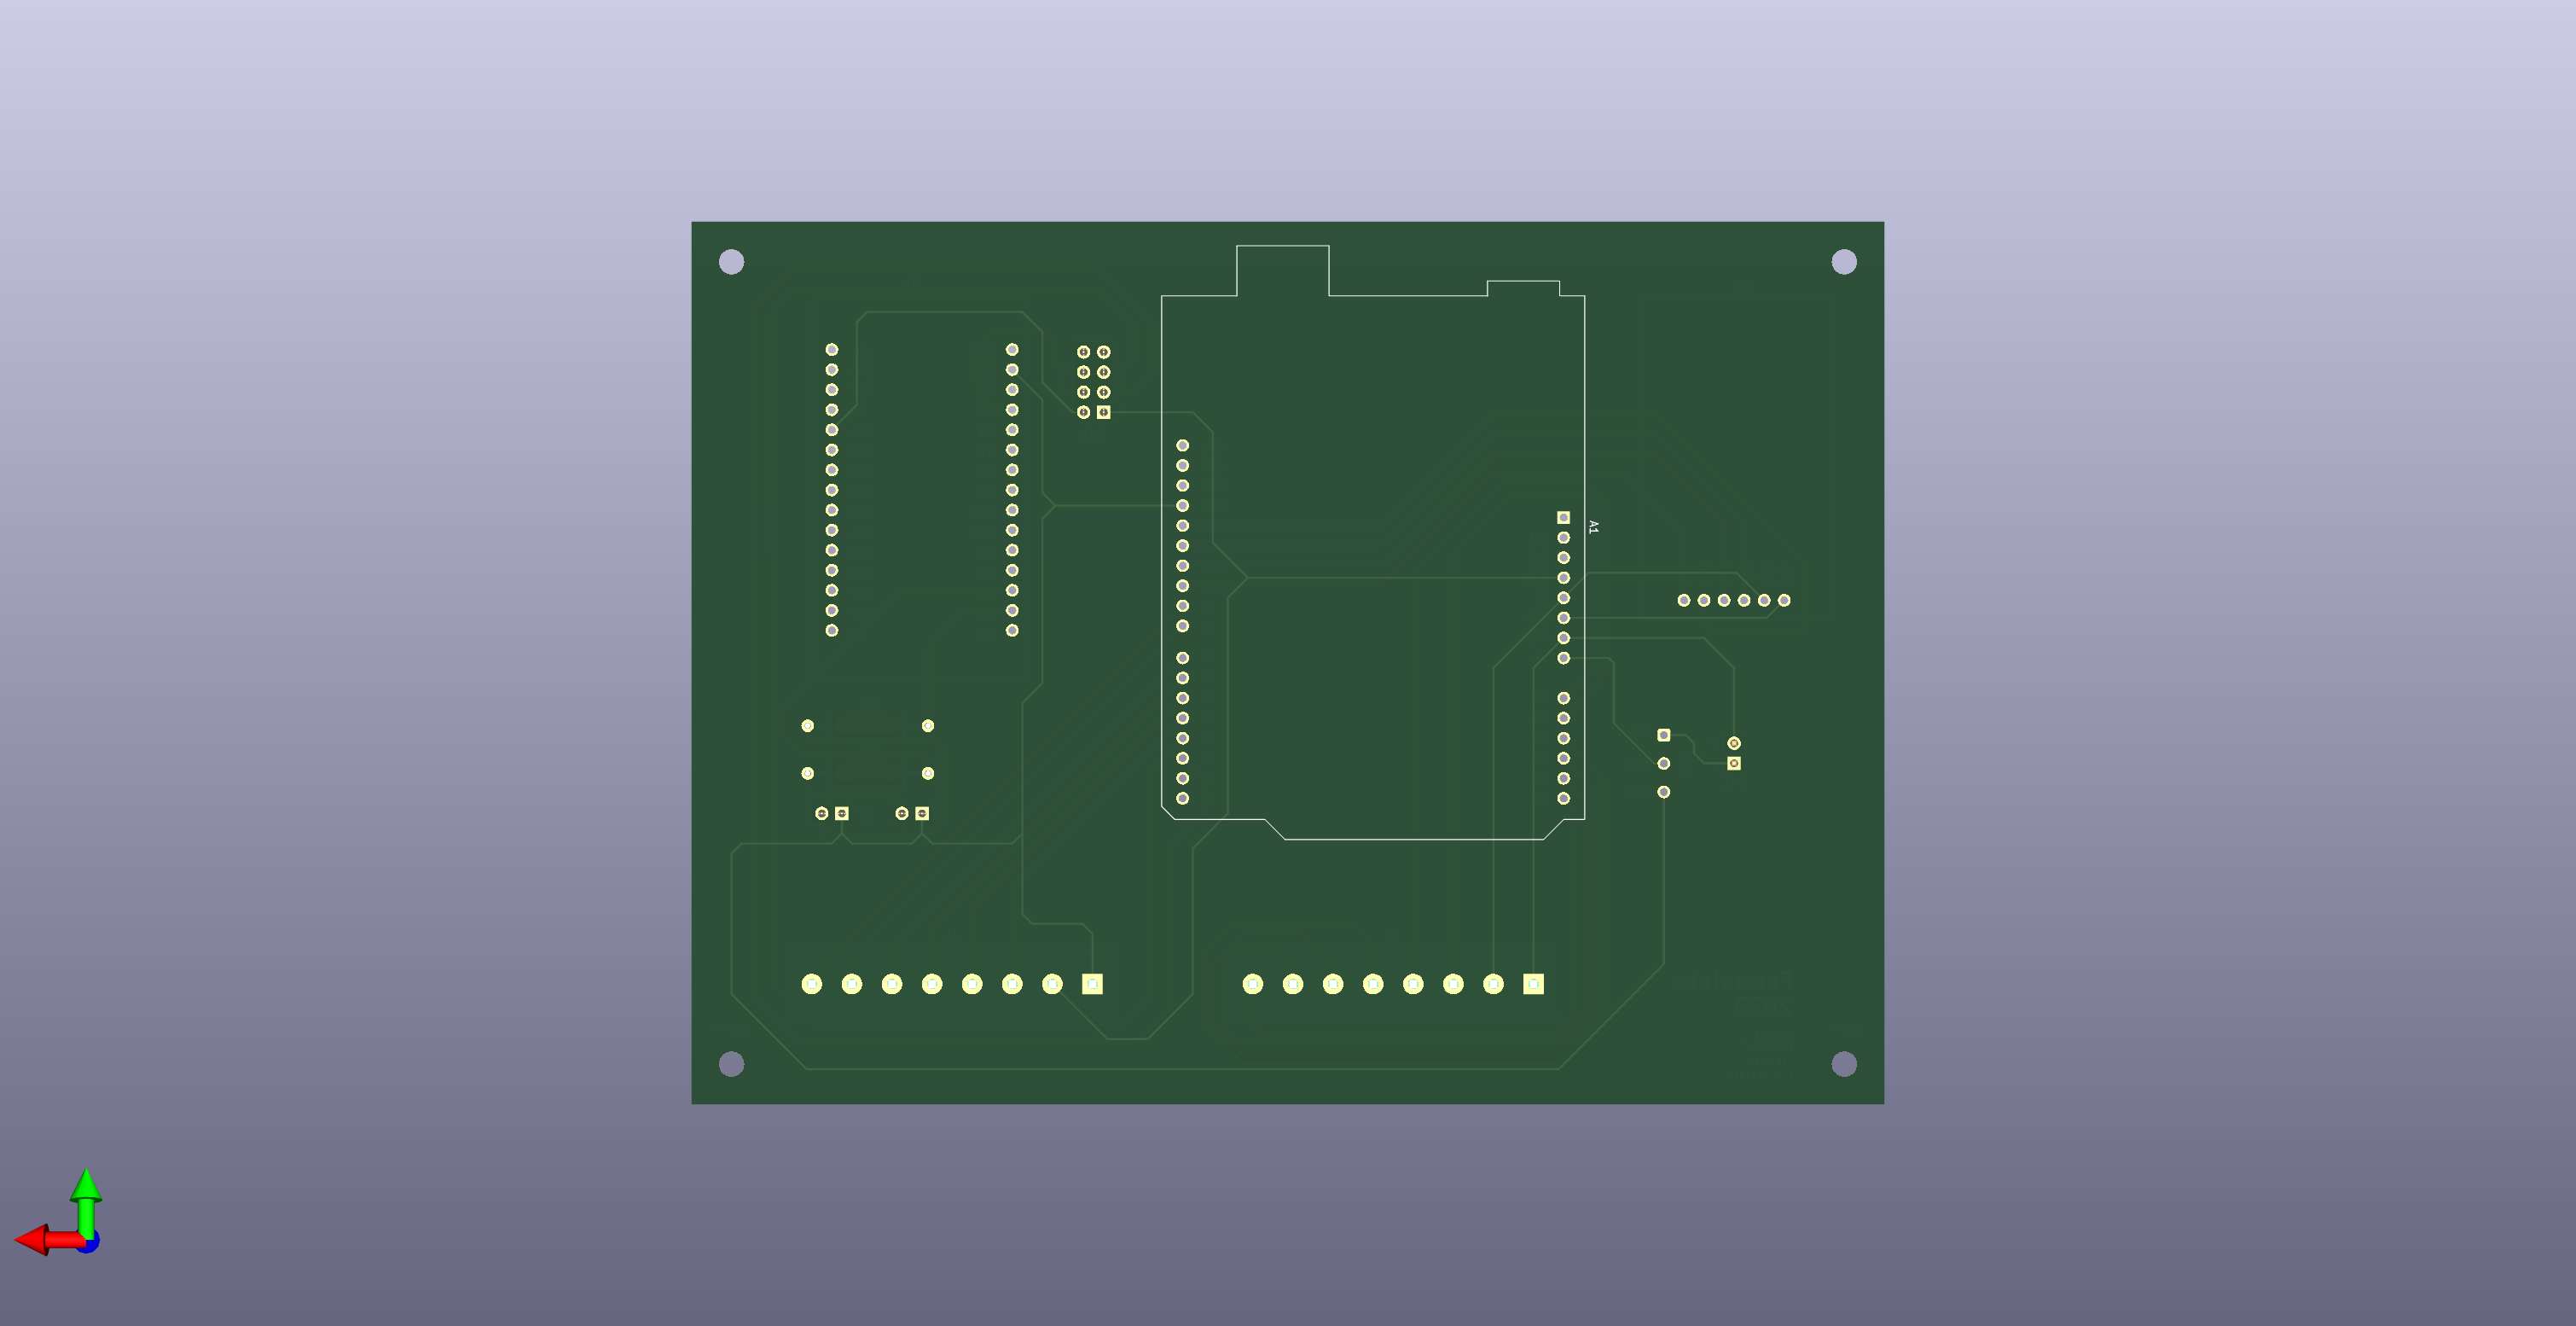
\includegraphics[width=1.0\textwidth]{PCB_Back_View}
  \caption{Bottom view of the PCB}
  \end{center}
  \end{figure}
  \newpage

\section{Communication Protocols}
N/A


\newpage
\section{Reflection}
\subsection{Wireless Communication}
\begin{enumerate}
  \item Some of the limitations of our device would be the range that our device can connect wirelessly. We are currently using an ESP8266 NodeMCU as the wireless module for our device, it acts as an access point and and broadcasts a network which our PC connects to. The NodeMCU operates on a 2.4GHz wifi network which does have long range but if we had unlimited resources we could have used another wireless protocol like LoRaWAN. Using a LoRaWAN connection or something similar could extend the wireless range of our device by a significant amount.
  \item An alternate method of connecting to our device would be to use a wireless hub. An external power router could have been used to connect our PC and device to, this would increase the range of the device and also simplify the connecting in our desktop application. The draw back of this solution would be that it requires an external router which would would need a direct ethernet connection. McMaster UTS blocks external router access on campus which would not make this solution feasible. Another method we considered was connecting our WiFi module to McMasters WiFi network, this would solve the range issue as campus wifi is broadly available around campus. There were two main issues with this solution, connecting to McMasters wifi would be complex as it requires a second layer of security to connect to it and also everytime the device would connect to wifi the IP address would change. The benefit of the currenlty implemented solution is that the IP address is static which means connecting to the device would not change. 
  
\end{enumerate}

\subsection{Application GUI}
\begin{enumerate}
  \item Some of the limitations of our device would be the range that our device can connect wirelessly. We are currently using an ESP8266 NodeMCU as the wireless module for our device, it acts as an access point and broadcasts a network to which our PC connects. The NodeMCU operates on a 2.4GHz wifi network which does have a long-range but if we had unlimited resources we could have used another wireless protocol like LoRaWAN. Using a LoRaWAN connection or something similar could extend the wireless range of our device by a significant amount.
  \item An alternate method of connecting to our device would be to use a wireless hub. An external power router could have been used to connect our PC and device, this would increase the range of the device and also simplify the connecting in our desktop application. The drawback of this solution would be that it requires an external router which would need a direct ethernet connection. McMaster UTS blocks external router access on campus which would not make this solution feasible. Another method we considered was connecting our WiFi module to McMasters WiFi network, this would solve the range issue as campus wifi is broadly available around campus. There were two main issues with this solution, connecting to McMasters wifi would be complex as it requires a second layer of security to connect to it, and also every time the device would connect to wifi the IP address would change. The benefit of the currently implemented solution is that the IP address is static which means connecting to the device would not change.
\end{enumerate}

\subsection{PCB Layout}
\begin{enumerate}
  \item Minimal PCB optimization was made to the layout. Primarily due to the time limitation of a lengthy and costly design, manufacture, test cycle for each PCB iteration, it was not feasible to optimize important PCB characteristics such as the absolute minimal layout size, noise minimization, and maximum structural rigidity. As a result, the team focused on achieving the functional solution in the shortest amount of time which limited optimization considerations.
  \item A breadboard circuit with jumper cables and pin header connections was a simpler alternative solution to a PCB design. The breadboard circuit had some benefits such as the inexpensive monetary cost to design, manufacture, and test, and the short time to complete a complete circuit iteration. With that said however, the breadboard circuit lacked the ability to create robust wire connections between components and the ability to design a circuit with a smaller physical footprint. As a result, a PCB layout which functionally replaced the breadboard circuit was chosen as the ability to design a physically smaller circuit with rigid connections through soldered points and terminal blocks was possible.
\end{enumerate}

\subsection{Dashboard}
\begin{enumerate}
  \item Minimal design optimization for the dashboard was made since the data that will be visualized is hard to make without the product being fully designed. We have used data that we believe will be similar to the data recieved by our product but there is no guarantee that the dashboard we desgined will be fully optimized for our product when it is fully function. 
  \item An alternate method would've been to design a website which would store all the data in a table for the user. The user would then graph this table in the format they please by copying and putting the data into a table that graphs the results. This method allowed for a more robust visualizing and storing of test data. This method although being more robust does come with flaws since it would require the user to already to take extra steps to visualize there data making rather inconvienent for them. We ultimately came to the decision to use Power Bi to visualize the data since it will seemlessly visualize the data as its being recieved by the database. Even though the same flexibility and robustness is not there it was determined to be a better option because of how compabatible Power Bi and databases are.
\end{enumerate}










\wss {
The information in this section will be used to evaluate the team members on the
graduate attribute of Problem Analysis and Design.  Please answer the following questions:

\begin{enumerate}
  \item What are the limitations of your solution?  Put another way, given
  unlimited resources, what could you do to make the project better? (LO\_ProbSolutions)

  \item Give a brief overview of other design solutions you considered.  What
  are the benefits and tradeoffs of those other designs compared with the chosen
  design?  From all the potential options, why did you select documented design?
  (LO\_Explores)
\end{enumerate} }


\end{document}